\documentclass{standalone}
\usepackage{pgfplots}
\pgfplotsset{compat=1.18}


\begin{document}
	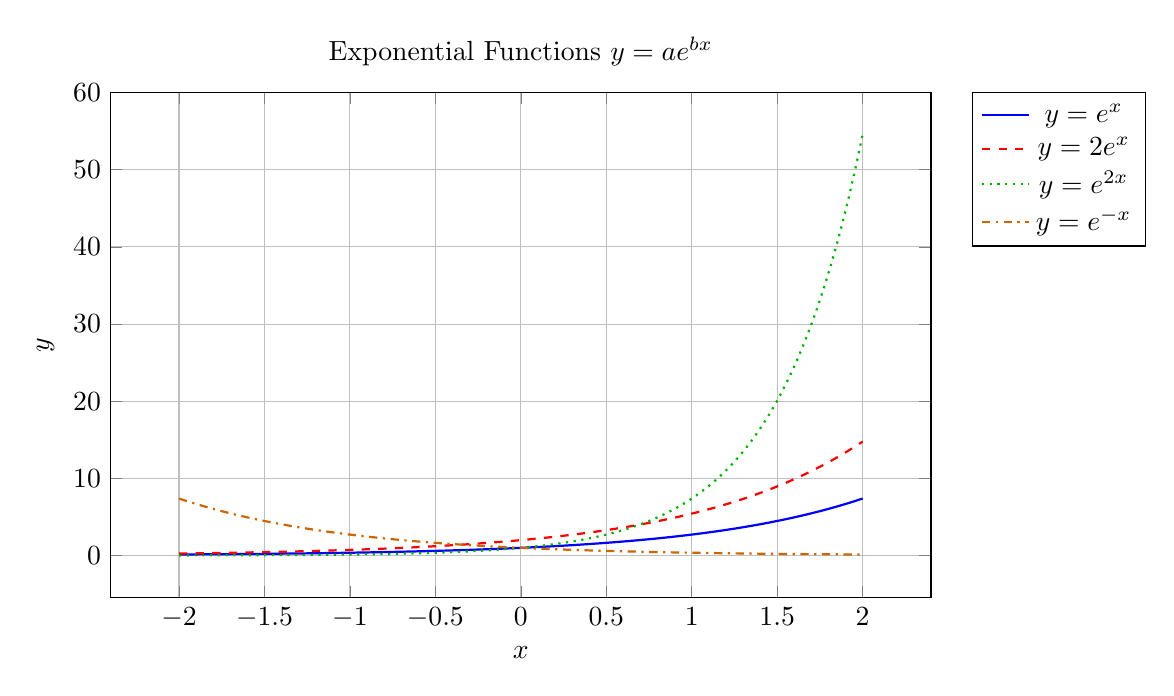
\begin{tikzpicture}
		\begin{axis}[
			title={Exponential Functions $y = a e^{bx}$},
			xlabel={$x$},
			ylabel={$y$},
			grid=major,
			legend style={at={(1.05,1)}, anchor=north west},
			width=12cm,
			height=8cm,
			]
			
			% y = e^x
			\addplot[domain=-2:2, samples=200, thick, blue]{exp(x)};
			\addlegendentry{$y = e^{x}$}
			
			% y = 2e^x
			\addplot[domain=-2:2, samples=200, thick, red, dashed]{2*exp(x)};
			\addlegendentry{$y = 2e^{x}$}
			
			% y = e^{2x}
			\addplot[domain=-2:2, samples=200, thick, green!70!black, 
			dotted]{exp(2*x)};
			\addlegendentry{$y = e^{2x}$}
			
			% y = e^{-x}
			\addplot[domain=-2:2, samples=200, thick, orange!80!black, dash 
			dot]{exp(-x)};
			\addlegendentry{$y = e^{-x}$}
			
		\end{axis}
	\end{tikzpicture}
\end{document}